
\documentclass[11pt]{article}

\usepackage[margin=1in]{geometry}   % See geometry.pdf to learn the layout options. There are lots.
\geometry{letterpaper}              % ... or a4paper or a5paper or ... 

\DeclareRobustCommand{\subtitle}[1]{\\#1}
\usepackage{graphicx}
\usepackage{enumitem}
\usepackage{pdfpages}

\usepackage[colorlinks=true]{hyperref}
\hypersetup{
    colorlinks = true,
    citecolor=blue,
    linkcolor=blue,
    urlcolor=blue
}    
% \newcommand\redout{\bgroup\markoverwith
% {\textcolor{red}{\rule[.5ex]{2pt}{0.4pt}}}\ULon}

\usepackage[nolist]{acronym}        % They are defined in the text. jhrg 5/28/26
%\ifthenelse{\value{AcronymNewPage}=1}
%    {\pagebreak}
{\bigskip}
    {}

%\ifthenelse{\value{AcronymSection}=1}
%    {\section{Acronyms}\label{Acronym-List}}
%    {\centerline{\bf Acronyms}\label{Acronym-List}
%}
  
{\begin{acronym}[(A)ATSR]
\newcommand{\textsmaller}[1]{{\small #1}}
\newcommand{\smaller}[1]{{\small #1}}
\newcommand{\larger}[1]{{\large #1}}
%\parskip 0pt
%\acro{(A)ATSR}{one or all of \textsmaller{ATSR}, \textsmaller{ATSR-2} and \textsmaller{AATSR}}
\acro{(A)ATSR}{one or all of \textsmaller{ATSR}, \textsmaller{ATSR-2} and \textsmaller{AATSR}}
\acro{AATSR}{Advanced Along Track Scanning Radiometer}
\acro{ACC}{Antarctic Circumpolar Current}
\acro{ACCESS}{Advancing Collaborative Connections for Earth System Science}
\acro{ACL}{Access Control List}
\acro{ACSPO}{Advanced Clear Sky Processor for Oceans}
\acro{ADA}{Automatic Detection Algorithm}
\acro{ADCP}{Acoustic Doppler Current Profiler}
\acro{ADT}{absolute dynamic topography}
\acro{AESOP}{Assessing the Effects of Submesoscale Ocean Parameterizations}
\acro{AGU}{American Geophysical Union}
\acro{AI}{Artificial Intelligence}
\acro{AIRS}{Atmospheric Infrared Sounder}
\acro{AIS}{Ancillary Information Service}
\acro{AIST}{Advanced Information Systems Techonology}
\acro{AISR}{Applied Information Systems Research}
\acro{ADL}{Alexandria Digital Library}
\acro{API}{Application Program Interface}
\acro{APL}{Applied Physics Laboratory}
\acro{API}{Application Program Interface}
\acro{AMSR}{Advanced Microwave Scanning Radiometer}
\acro{AMSR2}{Advanced Microwave Scanning Radiometer 2}
\acro{AMSR-E}{Advanced Microwave Scanning Radiometer - \textsmaller{EOS}}
\acro{ANN}{ Artificial Neural Network}
\acro{AOOS}{Alaska Ocean Observing System}
\acro{APAC}{Australian Partnership for Advanced Computing}
\acro{APDRC}{Asia-Pacific Data-Research Center}
%\acro{ARC}{\acs{ATSR} Reprocessing for Climate}
\acro{ARC}{{\smaller ATSR} Reprocessing for Climate}
\acro{ASCII}{American Standard Code for Information Interchange}
\acro{AS}{Aggregation Server}
\acro{ASFA}{Aquatic Sciences and Fisheries Abstracts}
\acro{ASTER}{Advanced Spaceborne Thermal Emission and Reflection Radiometer}
%{ -- \it http://asterweb.jpl.nasa.gov}
\acro{ATBD}{Algorithm Theoretical Basis Document}
\acro{ATree}{alternating decision tree}
\acro{ATSR}{Along Track Scanning Radiometer}
\acro{ATSR-2}{Second \textsmaller{ATSR}}
\acro{AVISO}{Archiving, Validation and Interpretation of Satellite Oceanographic Data}
\acro{ANU}{Australian National University}
\acro{AVHRR}{Advanced Very High Resolution Radiometer}
\acro{AWS}{Amazon Web Services}
\acro{AzC}{Azores Current}

\acro{BAA}{Broad Agency Announcement}
\acro{BAO}{bi-annual oscillation}
\acro{BES}{Back-End Server}
\acro{BMRC}{Bureau of Meteorology Research Centre}
\acro{BOM}{Bureau of Meteorology}
\acro{BT}{brightness temperature}
\acro{BUFR}{Binary Universal Format Representation}
%{ -- \it http://www.wmo.ch/web/www/WDM/Guides/Guide-on-DataMgt-1.htm}

\acro{CAN}{Cooperative Agreement Notice}
\acro{CAS}{Community Authorization Service}
\acro{CCA}{Cayula-Cornillon Algoritm}
\acro{CCI}{Climate Change Initiative}
\acro{CCLRC}{Council for the Central Laboratory of the Research Councils}
%{ --- \it http://www.cclrc.ac.uk/}
\acro{CCMA}{Center for Coastal Monitoring and Assessment}
\acro{CCS}{California Current System }
\acro{CCSM}{Community Climate System Model}
\acro{CCSR}{Center for Climate System Research}
\acro{CCV}{Center for Computation and Visualization}
\acro{CDAT}{Climate Data Analysis Tools}
\acro{CDC}{Climate Diagnostics Center}
\acro{CDF}{Common Data Format}
\acro{CDR}{Common Data Representation}
\acro{CEDAR}{Coupled Energetic and Dynamics and Atmospheric Regions}
%{ -- \it http://cedarweb.hao.ucar.edu/}
\acro{CEOS}{Committee on Earth Observation Satellites}
\acro{CERT}{Computer Emergency Response Team}
\acro{CenCOOS}{Central \& Northern California Ocean Observing System}
\acro{CF}{NetCDF Climate and Forecast Metadata Conventions}
\acro{CGI}{Common Gateway Interface}
%\acro{CHAP}{\textsmaller{CISL} \ac{HPC} Advisory Panel}
\acro{CHAP}{\textsmaller{CISL} High Performance Computing Advisory Panel}
\acro{CIFS}{Common Internet File System}
\acro{CICD}[CI/CD]{continuous integration and continuous delivery}
\acro{CIMSS}{Cooperative Institute for Meteorological Satellite Studies}
\acro{CIRES}{Cooperative Institute for Research (in) Environmental Sciences}
\acro{CISL}{Computational \& Information Systems Laboratory}
\acro{CLASS}{Comprehensive Large Array-data Stewardship System}
\acro{CLIVAR}{Climate Variability and Predictability}
\acro{CLS}{Collecte Localisation Satellites}
\acro{CME}{Community Modeling Effort}
\acro{CMS}{Centre de M\'et\'eorologie Spatiale}
\acro{CMR}{Common Metadata Repository}
\acro{CNN}{Convolutional Neural Network}
\acro{COA}{Climate Observations and Analysis}
\acro{COARDS}{Cooperative Ocean-Atmosphere Research Data Standard}
\acro{COAPS}{Center for Ocean-Atmospheric Prediction Studies}
\acro{COBIT}{Control Objectives for Information and related Technology}
%\acro{COCO}{\acs{CCSR} Ocean Component model}
\acro{COCO}{{\smaller CCSR} Ocean Component model}
\acro{CODAR}{Coastal Ocean Dynamics Applications Radar}
\acro{CODMAC}{Committee on Data Management, Archiving, and Computing}
\acro{Co-I}{Co-Investigator}
\acro{CORBA}{Common Object Request Broker Architecture}
\acro{COLA}{Center for Ocean-Land-Atmosphere Studies}
%{ -- \it http://grads.iges.org/cola.html}
\acro{CPU}{Central Processor Unit}
\acro{CRS}{Coordinate Reference System}
\acro{CSA}{Cambridge Scientific Abstracts}
\acro{CSC}{Coastal Services Center}
\acro{CSIS}{Center for Strategic and International Studies}
\acro{CSL}{Constraint Specification Language}
\acro{CSP}{Chermayeff, Sollogub and Poole, Inc.}
%{ -- \it http://csp-architects.com/contact.htm}
\acro{CSDGM}{Content Standard for Digital Geospatial Metadata}
%\acro{CTD}{Conductivity, Temperature and Salinity probes}
\acro{CTD}{Conductivity, Temperature and Salinity}
\acro{CVSS}{Common Vulnerability Scoring System}
\acro{CZCS}{Coastal Zone Color Scanner}

\acro{DAAC}{Distributed Active Archive Center}
\acro{DAARWG}{Data Archiving and Access Requirements Working Group}
\acro{DAP}{Data Access Protocol}
\acro{DAP4}{Data Access Protocol Version 4}
\acro{DAS}{Data set Attribute Structure}
\acro{DBMS}{Data Base Management System}
\acro{DBDB2}{Digital Bathymetric Data Base} 
\acro{DChart}{Dapper Data Viewer}
\acro{DDS}{Data Descriptor Structure}
\acro{DDX}{\textsmaller{XML} version of the combined \textsmaller{DAS} and \textsmaller{DDS}}
\acro{DFT}{Discrete Fourier Transform}
\acro{DIF}{Directory Interchange Format}
\acro{DISC}{Data and Information Services Center}
\acro{DIMES}{Diapycnal and Isopycnal Mixing Experiment:  Southern Ocean}
\acro{DMAC}{Data Management and Communications committee}
\acro{DMR++}{Data Model Response Plus Plus}
\acro{DMR}{Department of Marine Resources}
\acro{DMSP}{Defense Meteorological Satellite Program}
\acro{DoD}{Department of Defense}
\acro{DODS}{Distributed Oceanographic Data System}
%{ -- \it http://www.unidata.ucar.edu/packages/dods}
\acro{DOE}{Department of Energy}
%{ -- \it http://www.energy.gov}
\acro{DSP}{U. Miami satellite data processing software}
\acro{DSS}{direct statistical simulation}

\acro{EASy}{Environmental Analysis System}
%{ -- \it http://members.cox.net/fjobrien/global/layout/people.htm}
\acro{ECCO}{Estimating the Circulation and Climate of the Ocean}
\acro{ECCO2}{{\smaller  Estimating the Circulation and Climate of the Ocean} Phase II}
%\acro{ECS}{\textsmaller{EOSDIS} Core System}
\acro{ECHO}{Earth Observing System Clearinghouse}
\acro{ECMWF}{European Centre for Medium-range Weather Forecasting}
\acro{ECV}{Essential Climate Variable}
\acro{EDC}{Earthdata Cloud}
\acro{EDJ}{Equatorial Deep Jet}
\acro{EDFT}{Extended Discrete Fourier Transform}
\acro{EDMI}{Earth Data Multi-media Instrument}
%{ -- \newline \it http://www.newmediastudio.org/Homepage/TNMSHomeFramset.htm}
\acro{EEJ}{Extra-Equatorial Jet}
\acro{EIC}{Equatorial Intermediate Current}
\acro{EICS}{Equatorial Intermediate Current System}
\acro{EJ}{Equatorial Jets}
\acro{EKE}{eddy kinetic energy}
\acro{EMD}{Empirical Mode Decomposition}
\acro{EOF}{Empirical Orthogonal Function}
\acro{EOS}{Earth Observing System}
\acro{EOSDIS}{Earth Observing System Data Information System}
\acro{EPA}{Environmental Protection Agency}
\acro{EPSCoR}{Experimental Program to Stimulate Competitive Research}
\acro{EPR}{East Pacific Rise}
\acro{ERD}{Environmental Research Division}
\acro{ERS}{European Remote-sensing Satellite}
\acro{ESA}{European Space Agency}
\acro{ESDS}{Earth Science Data Systems}
\acro{ESDIS}{Earth Science Data and Information System Project}
%{ -- \it http://www.esdswg.org/}
\acro{ESDSWG}{Earth Science Data Systems Workign Group}
\acro{ESE}{Earth Science Enterprise}
\acro{ESG}{Earth System Grid}
%{ -- \it http://www.earthsystemgrid.org/}
\acro{ESG II}{Earth System Grid -- II}
%{ -- \it  http://www.earthsystemgrid.org}
\acro{ESIP}{Earth Science Information Partner}
%{ -- \it http://www.esipfed.org}
\acro{ESMF}{Earth System Modeling Framework}
%{ -- \texttt{http://www.esmf.ucar.edu}}
\acro{ESML}{Earth System Markup Language}
%{ -- \it http://esml.itsc.uah.edu/index.jsp}
\acro{ESP}{eastern South Pacfic}
\acro{ESRI}{Environmental Systems Research Institute}
%{-- \it http://www.esri.com}
\acro{ESR}{Earth and Space Research}
\acro{ETOPO}{Earth Topography}
\acro{EUC}{Equatorial Undercurrent}
\acro{EUMETSAT}{European Organisation for the Exploitation of Meteorological Satellites}
\acro{Ferret}{}
%{ -- \it http://ferret.pmel.noaa.gov/Ferret}

\acro{FASINEX}{Frontal Air-Sea Interaction Experiment}
\acro{FDS}{Ferret Data Server}
\acro{FFT}{Fast Fourier Transform}
\acro{FGDC}{Federal Geographic Data Committee}
%{ -- \it http://www.fgdc.gov}
\acro{FITS}{Flexible Image (or Interchange) Transport System}
\acro{FLOPS}{FLoating point Operations Per Second} 
\acro{FRTG}{Flow Rate Task Group}
\acro{FreeForm}{}
%{ -- \it http://www.ngdc.noaa.gov/seg/freeform/freeform.shtml}
\acro{FNMOC}{Fleet Numerical Meteorology and Oceanography Center}
\acro{FSU}{Florida State University}
\acro{FTE}{Full Time Equivalent}
\acro{ftp}[\normalsize  ftp]{File Transport Protocol}
\acro{FTP}[\normalsize  ftp]{File Transport Protocol}

\acro{GAC}{Global Area Coverage}
\acro{GAN}{Generative Adversarial Network}
\acro{GB}{GigaByte - $10^{9}$ bytes}
\acro{GCMD}{Global Change Master Directory}
%{ -- \it http://gcmd.nasa.gov}
\acro{GCM}{general circulation model}
\acro{GCOM-W1}{Global Change Observing Mission $1^{st}$ - Water}
\acro{GCOS}{Global Climate Observing System}
\acro{GDAC}{Global Data Assembly Center}
\acro{GDS}{\textsmaller{GrADS} Data Server}
\acro{GDS2}{GHRSST Data Processing Specification v2.0}
%{ -- \it http://grads.iges.org/grads/gds}
\acro{GEBCO}{General Bathymetric Charts of the Oceans}
\acro{GeoTIFF}{Georeferenced Tag Image File Format}
\acro{GEO-IDE}{Global Earth Observation Integrated Data Environment}
\acro{GES DIS}{Goddard Earth Sciences Data and Information Services Center}
\acro{GEMPACK}{General Equilibrium Modelling PACKage}
\acro{GEOSS}{Global Earth Observing System of Systems}
\acro{GFDL}{Geophysical Fluid Dynamics Laboratory}
\acro{GFD}{Geophysical Fluid Dynamics}
\acro{GHRSST}{Group for High Resolution Sea Surface Temperature}
\acro{GHRSST-PP}{\textsmaller{GODAE} High Resolution Sea Surface Temperature Pilot Project}
%{ -- \it  http://www.ghrsst-pp.org}
%\acro{GHRSST-PP}{\acs{GODAE}High Resolution Sea Surface Temperature Pilot Project}
%{ -- \it  http://www.ghrsst-pp.org}
\acro{GINI}{\textsmaller{GOES} Ingest and \textsmaller{NOAA/PORT} Interface}
\acro{GIS}{Geographic Information Systems} %{ -- \it http://www.gis.com}
\acro{Globus}{} %{ -- {http://www.globus.org}}
\acro{GMAO}{Global Modeling and Assimilation Office}
\acro{GML}{Geography Markup Language}
\acro{GMT}{Generic Mapping Tool}
\acro{GODAE}{Global Ocean Data Assimilation Experiment} %{ -- \it http://www.bom.gov.au/bmrc/ocean/GODAE}
\acro{GOES}{Geostationary Operational Environmental Satellites} %{ -- \it http://www.oso.noaa.gov/goes}
\acro{GOFS}{Global Ocean Forecasting System}
\acro{GoMOOS}{Gulf of Maine Ocean Observing System}
\acro{GOOS}{Global Ocean Observing System}
\acro{GOSUD}{Global Ocean Surface Underway Data}
\acro{GPFS}{ General Parallel File System}
\acro{GPU}{Graphics Processing Unit}
\acro{GRACE}{Gravity Recovery and Climate Experiment} %{ -- \it http://www.csr.utexas.edu/grace/spacecraft/config.html}
\acro{GRIB}{GRid In Binary} %{ -- \it http://www.wmo.ch/web/www/WDM/Guides/Guide-on-DataMgt-1.htm}
\acro{GrADS}{Grid Analysis and Display System} %{ -- \it http://grads.iges.org/grads/index.html}
\acro{GridFTP}{\textsmaller{FTP} with GRID enhancements}
\acro{GRIB}{GRid in Binary} %{ -- \it http://www.wmo.ch/web/www/DPS/grib-2.html}
\acro{GPS}{Global Positioning System}
\acro{GRU}{Gated Recurrent Unit}
\acro{GSFC}{Goddard Space Flight Center} %{ -- \it http://www.gsfc.nasa.gov}
\acro{GSI}{Grid Security Infrastructure}
\acro{GSO}{Graduate School of Oceanography}
\acro{GTSPP}{Global Temperature and Salinity Profile Program}
\acro{GUI}{Graphical User Interface}
\acro{GS}{Gulf Stream}

\acro{HAO}{High Altitude Observatory} %{ -- \it http://www.hao.ucar.edu/public/inside/data.html}
\acro{HLCC}{Hawaiian Lee Countercurrent}
\acro{HCMM}{Heat Capacity Mapping Mission}
\acro{HDF}{Hierarchical Data Format}
\acro{HDF-EOS}{Hierarchical Data Format - \textsmaller{EOS}} %{ -- \it http://hdfeos.gsfc.nasa.gov}
\acro{HEC}{High-End Computing}
\acro{HF}{High Frequency}
\acro{HGE}{High Gradient Event}
\acro{HPC}{High Performance Computing}
\acro{HPCMP}{High Performance Computing Modernization Program}
\acro{HPSS}{High Performance Storage System} %{ -- \it http://www.sdsc.edu/hpss/hpss1.html}
\acro{HR DDS}{High Resolution Diagnostic Data Set}
\acro{HRPT}{High Resolution Picture Transmission}
\acro{HTML}{Hyper Text Markup Language}
\acro{html}{Hyper Text Markup Language}
\acro{http}{the hypertext transport protocol}
\acro{HTTP}{Hyper Text Transfer Protocol}
\acro{HTTPS}{Secure Hyper Text Transfer Protocol} %\acro{http}{Hypertext Transport Protocol} It seems that the acronym is all caps.
\acro{HYCOM}{HYbrid Coordinate Ocean Model} %{ -- \it http://oceanmodeling.rsmas.miami.edu/hycom/}

\acro{I-band}{imagery resolution band}
\acro{IDD}{Internet Data Distribution}
\acro{IB}{Image Band}
\acro{IBL}{internal boundary layer}
\acro{IBM}{Internation Business Machines}
%{ -- \it http://www.ibm.com/us}
\acro{ICCs}{Intermediate Countercurrents}
\acro{IDE}{Integrated Development Environment}
\acro{IDL}{Interactive Display Language}
%{ -- \it  http://www.rsinc.com/idl/index.asp}
\acro{IDLastro}{\textsmaller{IDL} Astronomy User's Library}
\acro{IDV}{Integrated Data Viewer}
%{ -- \it http://my.unidata.ucar.edu/content/software/metapps/index.html}
\acro{IEA}{Integrated Ecosystem Assessment}
\acro{IEEE}{Institute (of) Electrical (and) Electronic Engineers}
%{ -- \it http://www.ieee.org/portal/index.jsp}
\acro{IETF}{Internet Engineering Task Force}
\acro{IFREMER}{Institut Fran\c{c}ais de Recherche pour l'Exploitation de la MER}
%\acro{IMF}{Interplanetary Magnetic Field}
\acro{IMAPRE}{El Instituto del Mar del Per\'u}
\acro{IMF}{Intrinsic Mode Function}
\acro{INLA}{Integrated Nested Laplace Approximations}
\acro{IOOS}{Integrated Ocean Observing System}
\acro{ISAR}{Infrared Sea surface temperature Autonomous Radiometer}
\acro{ISO}{International Organization for Standardization}
\acro{ISSTST}{Interim Sea Surface Temperature Science Team}
\acro{IT}{Information Technology}
\acro{ITCZ}{Intertropical Convergence Zone} 
\acro{IP}{Internet Provider}
\acro{IPCC}{Intergovernmental Panel on Climate Change}
\acro{IPRC}{International Pacific Research Center}
\acro{IR}{Infrared}
\acro{IRI}{International Research Institute for Climate and Society}
\acro{ISO}{International Standards Organization}

\acro{JASON}{JASON Foundation for Education}
%\acro{JASON}{NASA Altimeter}
%{ -- \it http://www.jason.org}
\acro{JAXA}{Japan Aerospace Exploration Agency}
\acro{JDBC}{Java Database Connectivity}
\acro{JFR}{Juan Fern\'andez Ridge}
\acro{JGOFS}{Joint Global Ocean Flux Experiment}
%{ -- \it http://puddle.mit.edu/datasys/jgsys.html}
\acro{JHU}{Johns Hopkins University}
\acro{JPL}{Jet Propulsion Laboratory}
\acro{JPSS}{Joint Polar Satellite System}
%{ -- \it http://www.jpl.nasa.gov}

\acro{KVL}{Keyword-Value List}
\acro{KML}{Keyhole Markup Language}
\acro{KPP}{K-Profile Parameterization}

\acro{LAC}{Local Area Coverage}
\acro{LAN}{Local Area Network}
\acro{LAS}{Live Access Server}
%{ -- \it http://www.ferret.noaa.gov/nopp/main.pl? }
\acro{LASCO}{Large Angle and Spectrometric Coronagraph Experiment}
\acro{LatMIX}{Scalable Lateral Mixing and Coherent Turbulence}
\acro{LDAP}{Lightweight Directory Access Protocol}
\acro{LDEO}{Lamont Doherty Earth Observatory}
\acro{LEAD}{Linked Environments for Atmospheric Discovery}
\acro{LEIC}{Lower Equatorial Intermediate Current}
\acro{LES}{Large Eddy Simulation}
\acro{LLC}{Latitude/Longitude/polar-Cap}
\acro{LLC4320}[LLC-4320]{\ac{LLC}-4320}
\acro{LLC2160}[LLC-2160]{\ac{LLC}-2160}
\acro{LLC1080}[LLC-1080]{\ac{LLC}-1080}
\acro{LHF}{Latent Heat Flux}
\acro{LST}{local sun time}
\acro{LSTM}{Long Short-Term Memory}
\acro{LTER}{Long Term Ecological Research Network}
\acro{LTSRF}{Long Term Stewardship and Reanalysis Facility}
\acro{LUT}{Look Up Table}

\acro{M-band}{moderate resolution band}
\acro{MABL}{marine atmospheric boundary layer}
\acro{MADT}{Maps of Absolute Dynamic Topography}
\acro{MapServer}{MapServer}
%{ -- \it http://mapserver.gis.umn.edu/}
\acro{MAT}{Metadata Acquisition Toolkit}
\acro{MATLAB}{}
%{ -- \it http://www.mathworks.com/products/}
\acro{MARCOOS}{Mid-Atlantic Coastal Ocean Observing System}
\acro{MARCOORA}{Mid-Atlantic Coastal Ocean Observing Regional Association}
\acro{MB}{MegaByte - $10^{6}$ bytes}
\acro{MCC}{Maximum Cross-Correlation}
\acro{MCMC}{Markov Chain Monte Carlo}
\acro{MCR}{\textsmaller{MATLAB} Component Runtime}
\acro{MCSST}{Multi-Channel Sea Surface Temperature}
\acro{MDT}{mean dynamic topography}
\acro{MDB}{Match-up Data Base}
\acro{MDOT}{mean dynamic ocean topography}
\acro{MEaSUREs}{Making Earth System data records for Use in Research Environments}
\acro{MERRA}{Modern Era Retrospective-Analysis for Research and Applications}
\acro{MERSEA}{Marine Environment and Security for the European Area}
\acro{MRF}{Markov Random Field}
\acro{MTF}{Modulation Transfer Function}
\acro{MICOM}{Miami Isopycnal Coordinate Ocean Model}
\acro{MIRAS}{Microwave Imaging Radiometer with Aperture Synthesis}
\acro{MITgcm}{{\smaller MIT} General Circulation Model}
\acro{MIT}{Massachusetts Institute of Technology}
\acro{mks}{meters, kilograms, seconds}
\acro{MLP}{Multilayer Perceptron}
\acro{MLSO}{Mauna Loa Solar Observatory}
%{ -- \it http://mslo.\ac{HAO}ucar.edu/}
\acro{MM5}{Mesoscale Model}
\acro{MMI}{Marine Metadata Initiative}
\acro{MMS}{Minerals Management Service}
\acro{MODAS}{Modular Ocean Data Assimilation System}
\acro{MODIS}{MODerate-resolution Imaging Spectroradiometer}
%{ -- \it http://modis.gsfc.nasa.gov}
\acro{MOU}{Memorandum of Understanding}
\acro{MCP}{Model Context Protocol}
\acro{MPARWG}{Metrics Planning and Reporting Working Group}
\acro{MSG}{Meteosat Second Generation}
\acro{MTPE}{Mission To Planet Earth}
\acro{MUR}{Multi-sensor Ultra-high Resolution}
\acro{MV}{Motor Vessel}

\acro{NAML}{National Association of Marine Laboratories}
\acro{NAHDO}{National Association of Health Data Organizations}
%{ -- \it http://www.nahdo.org}
\acro{NAS}{Network Attached Storage}
\acro{NASA}{National Aeronautics and Space Administration}
%{ -- \it http://www.nasa.gov}
\acro{NCAR}{National Center for Atmospheric Research}
%{ -- \it http://www.ncar.ucar.edu/ncar/index.html}
\acro{NCEI}{National Centers for Environmental Information}
\acro{NCEP}{National Centers for Environmental Prediction}
\acro{NCDC}{National Climatic Data Center}
\acro{NCDDC}{National Coastal Data Development Center}
\acro{NCL}{NCAR Command Language}
\acro{ncBrowse}{}
%{ -- \it http://www.epic.noaa.gov/java/ncBrowse}
\acro{NcML}{\textsmaller{netCDF} Markup Language}
\acro{NCO}{\textsmaller{netCDF} Operator}
\acro{NCODA}{Navy Coupled Ocean Data Assimilation}
\acro{NCSA}{National Center for Supercomputing Applications}
\acro{NDBC}{National Data Buoy Center}
\acro{NDVI}{Normalized Difference Vegetation Index}
\acro{NEC}{North Equatorial Current}
\acro{NECC}{North Equatorial Countercurrent}
\acro{NEFSC}{Northeast Fisheries Science Center}
\acro{NEIC}{North Equatorial Intermediate Current}
\acro{netCDF}{NETwork Common Data Format}
\acro{NEUC}{North Equatorial Undercurrent}
\acro{NGAP}{NASA Compliant General Application Platform}
\acro{NGDC}{National Geophysical Data Center}
%{ -- \it http://www.ngdc.noaa.gov}
\acro{NICC}{North Intermediate Countercurrent}
\acro{NIST}{National Institute of Standards and Technology}
\acro{NLSST}{Non-Linear Sea Surface Temperature}
\acro{NMFS}{National Marine Fisheries Service}
\acro{NMS}{New Media Studio}
%{ -- \it http://newmediastudio.org/Homepage/TNMSHomeFramset.htm}
\acro{NN}{Neural Network}
\acro{NOAA}{National Oceanic and Atmospheric Administration}
%{ -- \it http://www.noaa.gov}
\acro{NODC}{National Oceanographic Data Center}
\acro{NOGAPS}{Navy Operational Global Atmospheric Prediction System}
\acro{NOMADS}{\textsmaller{NOAA} Operational Model Archive Distribution System}
%{ -- \it http://www.ncdc.noaa.gov/oa/climate/nomads/nomads.html}
\acro{NOPP}{National Oceanographic Parternership Program}
%{ -- \it http://www.nopp.org}
\acro{NOS}{National Ocean Service}
\acro{NPP}{National Polar-orbiting Partnership}
\acro{NPOESS}{National Polar-orbiting Operational Environmental Satellite System}
\acro{NSCAT}{\textsmaller{NASA} SCATterometer}
%{ -- \it http://winds.jpl.nasa.gov}
%\acro{NSEN}{\acs{NASA}Science and Engineering Network}
\acro{NSEN}{\textsmaller{NASA} Science and Engineering Network}
\acro{NSF}{National Science Foundation}
%\acro{NSIPP}{\acs{NASA}Seasonal-to-Interannual Prediction Project}
\acro{NSIPP}{NASA Seasonal-to-Interannual Prediction Project}
\acro{NRA}{NASA Research Announcement}
\acro{NRC}{National Research Council}
\acro{NRL}{Naval Research Laboratory}
\acro{NSCC}{North Subsurface Countercurrent}
\acro{NSF}{National Science Foundation}
\acro{NSIDC}{National Snow and Ice Data Center}
\acro{NSPIRES}{\textsmaller{NASA} Solicitation and Proposal Integrated Review and Evaluation System}
\acro{NSSDC}{National Space Science Data Center}
\acro{NVODS}{National Virtual Ocean Data System}
%{ -- \it http://nvods.org}
\acro{NWP}{Numerical Weather Prediction}
\acro{NWS}{National Weather Service}

\acro{OBPG}{Ocean Biology Processing Group}
\acro{OB.DAAC}{Ocean Biology \textsmaller{DAAC}}
\acro{ODC}{\textsmaller{OPeNDAP} Data Connector}
\acro{OCAPI}{\textsmaller{OPeNDAP C API}}
\acro{ODSIP}{Open Data Services Invocation Protocol}
\acro{OFES}{Ocean Model for the Earth Simulator}
\acro{OCCA}{OCean Comprehensive Atlas}
\acro{OGC}{Open Geospatial Consortium}
%{ -- \it http://www.opengis.org}
\acro{OGCM}{ocean general circulation model}
\acro{OISSTv1}{Optimally Interpolated SST Version 1}
\acro{ONR}{Office of Naval Research}
\acro{OOPC}{Ocean Observation Panel for Climate}
\acro{OLCI}{Ocean Land Colour Instrument}
\acro{OLFS}{\textsmaller{OPeNDAP} Lightweight Front-end Server}
\acro{OPeNDAP}{Open source Project for a Network Data Access Protocol}
%{ -- \it http://opendap.org}
\acro{OPeNDAPg}{\textsmaller{GRID}-enabled \textsmaller{OPeNDAP} tools}
\acro{OpenGIS}{OpenGIS}
\acro{OSI SAF}{Ocean and Sea Ice Satellite Application Facility}
\acro{OSS}{Office of Space Science}
\acro{OSTM}{Ocean Surface Topography Mission }
\acro{OSU}{Oregon State University}
\acro{OS X}{}
\acro{OWL}{Web Ontology Language}
\acro{OWASP}{Open Web Application Security Project}

\acro{PBL}{planetary boundary layer}
\acro{PDistF}[PDF]{probability distribution function}
\acro{PDF}{probability density function}
\acro{PF}{Polar Front}
\acro{PFEL}{Pacific Fisheries Environmental Laboratory}
\acro{PI}{Principal Investigator}
\acro{PIV}{Particle Image Velocimetry}
\acro{PL}{Project Leader}
\acro{PM}{Project Member}
\acro{PMEL}{Pacific Marine Environmental Laboratory}
%{ -- \it http://pmel.noaa.gov}
\acro{POC}{particulate organic carbon}
\acro{PO.DAAC}{Physical Oceanography -- Distributed Active Archive Center}
%{ -- \it http://podaac.jpl.nasa.gov}
\acro{POP}{Parallel Ocean Program }
\acro{PSD}{Power Spectral Density}
\acro{PSPT}{Precision Solar Photometric Telescope}
\acro{PSU}{Pennsylvania State University}
\acro{PyDAP}{Python Data Access Protocol}
\acro{PV}{potential vorticity}

\acro{QC}{quality control}
\acro{QG}{quasi-geostrophic}
\acro{QuikSCAT}{Quick Scatterometer}
%{ -- \it http://winds.jpl.nasa.gov/missions/quikscat/quikindex.html}
\acro{QZJ}{quasi-zonal jet}

\acro{R2HA2}{Rescue \& Reprocessing of Historical AVHRR Archives }
\acro{RAFOS}{{\smaller SOFAR}, SOund Fixing And Ranging, spelled backward}
\acro{RAID}{Redundant Array of Independent Disks}
\acro{RAL}{Rutherford Appleton Laboratory}
\acro{RDF}{Resource Description Language}
\acro{REASoN}{Research, Education and Applications Solutions Network}
\acro{REAP}{Realtime Environment for Analytical Processing}
\acro{REU}{Research Experiences for Undergraduates}
\acro{RFA}{Research Focus Area}
\acro{RFI}{Radio Frequency Interference}
\acro{RFC}{Request For Comments}
\acro{R/GTS}{Regional/Global Task Sharing}
\acro{RSI}{Research Systems Inc.}
\acro{RISE}{Radiative Inputs from Sun to Earth}
\acro{rms}{root mean square}
\acro{RMI}{Remote Method Invocation}
\acro{RNN}{Recursive Neural Network}
\acro{ROMS}{Regional Ocean Modeling System}
\acro{ROSES}{Research Opportunities in Space and Earth Sciences}
\acro{RSMAS}{Rosenstiel School of Marine and Atmospheric Science}
\acro{RSS}{Remote Sensing Sytems}
\acro{RTM}{radiative transfer model}

%\acro{SACCF}{Southern \acs{ACC} Front}
\acro{SACCF}{Southern {\smaller ACC} Front}
\acro{SAC-D}[(SAC)-D]{Sat\'elite de Aplicaciones Cient\'ificas-D}
%\acro{SAF}{Satellite Application Facility}
\acro{SAF}{Subantarctic Front}
\acro{SAIC}{Science Applications International Corporation}
\acro{SANS}{SysAdmin, Audit, Networking, and Security}
\acro{SAR}{synthetic aperature radar}
\acro{SATMOS}{Service d'Archivage et de Traitement M\'et\'eorologique des Observations Spatiales}
\acro{SBE}{Sea-Bird Electronics}
\acro{SciDAC}{Scientific Discovery through Advanced Computing}
\acro{SCC}{Subsurface Countercurrent}
\acro{SCCWRP}{Southern California Coastal Water Research Project}
\acro{SDAC}{Solar Physics Data Analysis Center}
%\acro{SeaWinds}{NASA Scatterometer}
\acro{SDS}{Scientific Data Set}
\acro{SDSC}{San Diego Supercomputer Center}
\acro{SeaDAS}{\textsmaller{SeaWiFS} Data Analysis System}
\acro{SeaWiFS}{Sea-viewing Wide Field-of-view Sensor}
%\acro{SEC}{Sun Earth Connection}
\acro{SEC}{South Equatorial Current}
\acro{SECC}{South Equatorial Countercurrent}
\acro{SECDDS}{Sun Earth Connection Distributed Data Services}
\acro{SEEDS}{Strategic Evolution of \textsmaller{ESE} Data Systems}
%{ -- \it http://lennier.gsfc.nasa.gov/seeds}
\acro{SEIC}{South Equatorial Intermediate Current}
\acro{SEUC}{Southern Equatorial Undercurrent}
\acro{SEVIRI}{Spinning Enhanced Visible and Infra-Red Imager}
\acro{SeRQL}{SeRQL}
\acro{SGI}{Silican Graphics Incorporated}
%{ -- \it http://www.sgi.com}
\acro{SHF}{Sensible Heat Flux}
\acro{SICC}{South Intermediate Countercurrent}
\acro{SIED}{single image edge detection}
\acro{SIPS}{Science Investigator--led Processing System}
\acro{SIR}{Scatterometer Image Reconstruction}
\acro{SISTeR}{Scanning Infrared Sea Surface Temperature Radiometer}
\acro{SLA}{sea level anomaly}
\acro{SMAP}{Soil Moisture Active Passive}
\acro{SMMR}{Scanning Multichannel Microwave Radiometer}
\acro{SMOS}{Soil Moisture and Ocean Salinity}
\acro{SMTP}{Simple Mail Transfer Protocol}
\acro{SOAP}{Simple Object Access Protocol}
\acro{SOEST}{School of Ocean and Earth Science and Technology}
\acro{SOFAR}{SOund Fixing And Ranging}
\acro{SOFINE}{Southern Ocean Finescale Mixing Experiment}
\acro{SOHO}{Solar and Heliospheric Observatory}
\acro{SPARC}{Space Physics and Aeronomy Research Collaboratory}
%{ -- \it http://intel.si.umich.edu/SPARC/}
\acro{SPARQL}{Simple Protocol and \textsmaller{RDF} Query Language}
\acro{SPASE}{Space Physics Archive Search Engine}
\acro{SPCZ}{South Pacific Convergence Zone}  
\acro{SPDF}{Space Physics Data Facility}
\acro{SPDML}{Space Physics Data Markup Language}
%{ -- \it http://sd-www.jhuapl.edu/SPDML/}
\acro{SPG}{Standards Process Group}
%{ -- \it http://www.esdswg.org/spg/}
\acro{SQL}{Structured Query Language}
\acro{SSCC}{South Subsurface Countercurrent}
\acro{SSL}{Secure Sockets Layer}
\acro{SSO}{Single sign-on}
\acro{SSES}{Single Sensor Error Statistics}
\acro{SSH}{sea surface height}
%\acro{SSHA}{\ac{SSH} anomaly}
\acro{SSHA}{sea surface height anomaly}
\acro{SSMI}{Special Sensor Microwave/Imager}
\acro{SST}{sea surface temperature}
\acro{SSS}{sea surface salinity}
\acro{SSTST}{Sea Surface Temperature Science Team}
\acro{STEM}{science, technology, engineering and mathematics}
\acro{STL}{Standard Template Library}
\acro{STCZ}{Subtropical Convergence Zone}
\acro{STGP}{Space-Time Gaussian Processes}
\acro{Suomi-NPP}[{\larger Suomi}-NPP]{Suomi-\acl{NPP}}
\acro{SWEET}{Semantic Web for Earth and Environmental Terminology}
\acro{SWFSC}{Southwest Fisheries Science Center}
\acro{SWOT}{Surface Water and Ocean Topography}
\acro{SWRL}{Semantic Web Rule Language}
\acro{SubEx}{Submesoscale Experiment}
\acro{SURA}{Southeastern Universities Research Association}
\acro{SURFO}{Summer Undergraduate Research Fellowship Program in Oceanography}
\acro{SuperDARN}{Super Dual Auroral Radar Network}

\acro{TAMU}{Texas A\&M University}
\acro{TB}{TeraByte - $10^{12}$ bytes}
\acro{TCASCV}{Technology Center for Advanced Scientific Computing and Visualization}
%{ -- \newline \it http://www.cascv.brown.edu/aboutus.html}
\acro{TCP}{Transmission Control Protocol}
\acro{TCP/IP}{Transmission Control Protocol/Internet Protocol}
\acro{TDS}{\textsmaller{THREDDS} Data Server}
\acro{TEX}{external temperature or T-External}
\acro{THREDDS}{Thematic Realtime Environmental Data Distributed Services}
%{ -- \newline \it http://my.unidata.ucar.edu/content/projects/THREDDS/index.html}
\acro{TIDI}{\textsmaller{TIMED} Doppler Interferometer}
\acro{TIFF}{Tag Image File Format}
\acro{TIMED}{Thermosphere, Ionosphere, Mesosphere, Energetics and Dynamics}
\acro{TLS}{Transport Layer Security}
\acro{TRL}{Technology Readiness Level}
\acro{TMI}{\textsmaller{TRMM} Microwave Imager}
\acro{TOPEX/Poseidon}{TOPography EXperiment for Ocean Circulation/Poseidon}
\acro{TRMM}{Tropical Rainfall Measuring Mission}
%{ -- \it http://trmm.gsfc.nasa.gov/}
\acro{TSG}{thermosalinograph}

\acro{UCAR}{University Corporation for Atmospheric Research}
%{ -- \it http://www.ucar.edu}
\acro{UCSB}{University of California, Santa Barbara}
\acro{UCSD}{University of California, San Diego}
\acro{UCT}{Coordinated Universal Time}
\acro{uCTD}{Underway Conductivity, Temperature and Salinity or Underway \acs{CTD}}
\acro{UDDI}{Universal Description, Discovery and Integration}
\acro{UMiami}{University of Miami}
\acro{Unidata}{}
%{ -- \it http://unidata.ucar.edu}
\acro{URI}{University of Rhode Island}
%{ -- \it http://www.uri.edu}
\acro{UPC}{Unidata Program Committee}
\acro{URL}{Uniform Resource Locator}
\acro{US}{United States}
\acro{USGS}{United States Geological Survey}
\acro{UTC}{Coordinated Universal Time}
\acro{UW}{University of Washington}

\acro{VCDAT}{Visual Climate Data Analysis Tools}
\acro{VIIRS}{Visible-Infrared Imager-Radiometer Suite}
\acro{VIRS}{Visible and Infrared Scanner}
\acro{VR}{Virtual Reality}
\acro{VSTO}{Virtual Solar-Terrestrial Observatory}

\acro{WCOM-W1}{Global Change Observation Mission $1^{st}$ - Water}
\acro{WCR}{warm core ring}
\acro{WCS}{Web Coverage Service}
%{ -- \it http://www.ogcnetwork.org}
\acro{WCRP}{World Climate Research Program}
\acro{WFS}{Web Feature Service}
%{ -- \it http://www.ogcnetwork.org}
\acro{WMS}{Web Map Service}
%{ -- \it http://www.ogcnetwork.org}
\acro{W3C}{World Wide Web Consortium}
\acro{WJ}{Wyrtki Jets}
\acro{WHOI}{Woods Hole Oceanographic Institution}
\acro{WKB}{Well Known Binaries}
\acro{WIMP}{Windows, Icons, Menus, and Pointers}
\acro{WMO}{World Meteorological Organisation}
\acro{WIS}{World Meteorological Organisation Information System}
\acro{WOA05}{World Ocean Atlas 2005}
\acro{WOCE}{World Ocean Circulation Experiment}
\acro{WP-ESIP}{Working Prototype Earth Science Information Partner}
\acro{WRF}{Weather \& Research Forecasting Model}
\acro{WSDL}{Web Services Description Language}
\acro{WSP}{western South Pacfic}
\acro{WWW}{World Wide Web}

\acro{XBT}{Expendable BathyThermograph}
\acro{XML}{Extensible Markup Language}
%{ -- \it http://www.w3.org/XML}
\acro{XRAC}{eXtreme Digital Request Allocation Committee}
\acro{XSEDE}{Extreme Science and Engineering Discovery Environment}

\acro{YAG}{yttrium aluminium garnet}

\end{acronym}
}

\clearpage

%\renewcommand*{\acsfont}[1]{\textsmaller{#1}}

\newcommand{\ai}{\ac{AI}}
\newcommand{\ais}{\acp{AI}}
\newcommand{\amsre}{\ac{AMSR-E}}
\newcommand{\amsrtwo}{\ac{AMSR2}}
\newcommand{\amsreshort}{\acs{AMSR-E}}
%\newcommand{\aatsr}{\ac{(A)ATSR}}
\newcommand{\aatsr}{\ac{AATSR}}
\newcommand{\ann}{\ac{ANN}}
\newcommand{\anns}{\acp{ANN}}
\newcommand{\avhrr}{\ac{AVHRR}}
\newcommand{\avhrrshort}{\acs{AVHRR}}
\newcommand{\avhrrs}{\acp{AVHRR}}
\newcommand{\aws}{\ac{AWS}}

\newcommand{\bitone}{Bit~1}
\newcommand{\bittwo}{Bit~2}
\newcommand{\bitthree}{Bit~3}
\newcommand{\bitfour}{Bit~4}
\newcommand{\bitfive}{Bit~5}
\newcommand{\bitsix}{Bit~6}
\newcommand{\bitseven}{Bit~7}
\newcommand{\biteight}{Bit~8}
\newcommand{\bitnine}{Bit~9}
\newcommand{\bitten}{Bit~10}
\newcommand{\biteleven}{Bit~11}
\newcommand{\bittwelve}{Bit~12}
\newcommand{\bitthirteen}{Bit~13}
\newcommand{\bitfourteen}{Bit~14}
\newcommand{\bitfifteen}{Bit~15}
\newcommand{\bitsixteen}{Bit~16}
\newcommand{\bt}{\ac{BT}}
\newcommand{\btplural}{\acp{BT}}

\newcommand{\cms}{\ac{CMS}}
\newcommand{\cnn}{\ac{CNN}}
\newcommand{\cnns}{\acp{CNN}}

%\newcommand{\dataset}{data set}
%\newcommand{\datasets}{data sets}
\newcommand{\degree}{$^\circ$}

\newcommand{\ecco}{\acs{ECCO2}}
\newcommand{\eightteenghz}{$18.7\,{\rm GHz}$}
\newcommand{\eightynineghz}{$89.0\,{\rm GHz}$}
\newcommand{\Excel}{\textsmaller Excel}
\newcommand{\elevenbyelven}{$11\times11$}
\newcommand{\esdis}{\acs{ESDIS}}

\newcommand{\fiftybyfifty}{$56\times56$}
\newcommand{\fiftybyfiftykm}{$56\times56\,\mbox{km}^2$}
\newcommand{\seventybyfortykm}{$75\times45\,\mbox{km}^2$}
\newcommand{\fiftykm}{$50\,{\rm km}$}
\newcommand{\fiftysixkm}{$56\,{\rm km}$}
\newcommand{\fivebyfive}{$5\times5$}
\newcommand{\footprint}{$45\times75$\,km$^{2}$}
\newcommand{\fourkm}{4~km}

\newcommand{\gac}{\ac{GAC}}
\newcommand{\gan}{\ac{GAN}}
\newcommand{\gans}{\acp{GAN}}
\newcommand{\ghrsst}{\ac{GHRSST}}
\newcommand{\gui}{\ac{GUI}}
\newcommand{\guis}{\acp{GUI}}

\newcommand{\hycom}{\ac{HYCOM}}

\newcommand{\iband}{{\smaller I}-band}
\newcommand{\ibands}{{\smaller I}-bands}
\newcommand{\indicateSpace}{$_{\color{black}\sqcap}$}
\newcommand{\ItemAnswer}[1]{\item[]<.-> \smaller {\color{cyan} #1}}
\newcommand{\ItemAnswerAdvance}[1]{\item[]<+-> \smaller {\color{cyan} #1}}
\newcommand{\ItemCommandLine}[1]{\item[$>>$]<.-> \smaller {\color{orange} #1;}}
\newcommand{\ItemCommandLineAdvance}[1]{\item[$>>$]<+-> \smaller {\color{orange} #1;}}
\newcommand{\ItemCommandLineIndent}[1]{\item[$>>$]<.-> \hspace{.1in} \smaller {\color{orange} #1;}}
\newcommand{\ItemCommandLineIndentNoSemicolon}[1]{\item[$>>$]<.-> \hspace{.1in} \smaller {\color{orange} #1}}
\newcommand{\ItemCommandLineNoSemicolon}[1]{\item[$>>$]<.-> \smaller {\color{orange} #1}}
\newcommand{\ItemCommandLineNoSemicolonAdvance}[1]{\item[$>>$]<+-> \smaller {\color{orange} #1}}

\newcommand{\ItemDebugCommandLine}[1]{\item[k$>>$]<.-> \smaller {\color{orange} #1}}
\newcommand{\ItemDebugCommandLineAdvance}[1]{\item[k$>>$]<+-> \smaller {\color{orange} #1}}
\newcommand{\ItemDebugCommandLineNoSemicolon}[1]{\item[k$>>$]<.-> \smaller {\color{orange} #1}}
\newcommand{\ItemDebugCommandLineNoSemicolonAdvance}[1]{\itemk[$>>$]<+-> \smaller {\color{orange} #1}}

\newcommand{\ItemEditor}[1]{\item[]<.-> \smaller {\color{orange} #1;}}
\newcommand{\ItemEditorIndent}[1]{\item[]<.-> \hspace{.1in} \smaller {\color{orange} #1;}}
\newcommand{\ItemEditorAdvance}[1]{\item[]<+-> \smaller {\color{orange} #1;}}
\newcommand{\ItemEditorNoSemicolon}[1]{\item[]<.-> \smaller {\color{orange} #1}}
\newcommand{\ItemEditorNoSemicolonIndent}[1]{\item[]<.-> \hspace{.1in} \smaller {\color{orange} #1}}
\newcommand{\ItemEditorNoSemicolonAdvance}[1]{\item[]<+-> \smaller {\color{orange} #1}}
\newcommand{\ItemEditorIndentNoSemicolon}[1]{\item[]<.-> \hspace{.1in} \smaller {\color{orange} #1}}
\newcommand{\ItemEditorIndentNoSemicolonAdvance}[1]{\item[]<+-> \hspace{.1in} \smaller {\color{orange} #1}}

\newcommand{\ItemOR}{\item<.->[] OR}
\newcommand{\ItemORAdvance}{\item<+->[] OR}
\newcommand{\ItemNoBullet}{\item<.->[] }
\newcommand{\ItemNoBulletAdvance}{\item<+->[] }
\newcommand{\ItemQuestion}[1]{\item[]<.-> \smaller {\color{magenta} #1}}
\newcommand{\ItemQuestionAdvance}[1]{\item[]<+-> \smaller {\color{magenta} #1}}
\newcommand{\ItemQuestionAnswer}[2]{\item[]<.-> \smaller {\color{magenta} #1} {\color{cyan} #1}}
\newcommand{\ItemQuestionAnswerAdvance}[2]{\item[]<.-> \smaller {\color{magenta} #1} {\color{cyan} #1}}

\newcommand{\ir}{\ac{IR}}

\newcommand{\jaxa}{\ac{JAXA}}

\newcommand{\llcone}{\acs{LLC}\textsmaller{1080}}
\newcommand{\llctwo}{\acs{LLC}\textsmaller{2160}}
\newcommand{\llcfour}{\acs{LLC}\textsmaller{4320}}
\newcommand{\Lfour}{\textsmaller{L4}}
\newcommand{\LfourP}{\textsmaller{L4P}}
\newcommand{\Lone}{\textsmaller{L1}}
\newcommand{\Loneb}{\textsmaller{L1b}}
\newcommand{\Lthree}{\textsmaller{L3}}
\newcommand{\LthreeP}{\textsmaller{L3P}}
\newcommand{\Ltwo}{{L2}}
\newcommand{\LtwoP}{\textsmaller{L2P}}
\newcommand{\LtwoPcore}{\textsmaller{L2Pcore}}

\newcommand{\mband}{{\smaller M}-band}
\newcommand{\mbands}{{\smaller M}-bands}
\newcommand{\MM}{\textsmaller{MMNS}\ }
\newcommand{\modis}{\ac{MODIS}}
\newcommand{\modisshort}{\acs{MODIS}}
\newcommand{\msg}{\ac{MSG}}

\newcommand{\nasa}{\acs{NASA}}
\newcommand{\ngap}{\acs{NGAP}}
\newcommand{\ninekm}{9~km}
\newcommand{\ninebynine}{$9\times9$}
%\newcommand{\nn}{\acs{NN}}
\newcommand{\nn}{neural network}
\newcommand{\nns}{\acp{NN}}
\newcommand{\noaa}{\acs{NOAA}} 

\newcommand{\obpg}{\acs{OBPG}} 
\newcommand{\onekm}{1~km}
\newcommand{\opendap}{\acs{OPeNDAP}}

\newcommand{\podaac}{\ac{PO.DAAC}} 

\newcommand{\rms}{\ac{rms}}
\newcommand{\rnn}{\ac{RNN}}
\newcommand{\rnns}{\acp{RNN}}
\newcommand{\roms}{\ac{ROMS}}
\newcommand{\rss}{\ac{RSS}}

\newcommand{\sevenghz}{$7.30\,{\rm GHz}$}
\newcommand{\seviri}{\ac{SEVIRI}}
\newcommand{\sfm}{$750\,{\rm m}$}
\newcommand{\sied}{\ac{SIED}}
\newcommand{\sixghz}{$6.93\,{\rm GHz}$}
\newcommand{\ssh}{\ac{SSH}}
\newcommand{\sshs}{\acs{SSH}}
\newcommand{\sst}{\ac{SST}}
\newcommand{\sstfour}{\ac{SST}4}
\newcommand{\swot}{\ac{SWOT}}
\newcommand{\smap}{\ac{SMAP}}

\newcommand{\tenbyten}{$10\times10$\,km}
\newcommand{\tenbytenkm}{$10\times10\,\mbox{km}^2$}
\newcommand{\tenghz}{$10.65\,{\rm GHz}$}
\newcommand{\tenkm}{$10\,{\rm km}$}
\newcommand{\theband}{{\it the band}}
\newcommand{\thirtysixghz}{$36.5\,{\rm GHz}$}
\newcommand{\thirtybythirty}{$30\times30$}
\newcommand{\threebythree}{$3\times3$ pixel square}
\newcommand{\tmi}{\ac{TMI}}
\newcommand{\trl}{\ac{TRL}}
\newcommand{\tsfm}{$375\,{\rm m}$}
\newcommand{\twentyfivekm}{25~km}
\newcommand{\twentythreeghz}{$23.8\,{\rm GHz}$}

\newcommand{\uri}{\ac{URI}}

\newcommand{\viirs}{\ac{VIIRS}}
\newcommand{\viirsshort}{\acs{VIIRS}}

\newcommand{\xxx}{{\color{red}xxx}}

\usepackage{fontspec}               % Use the XeLaTeX compiler in Overleaf for 'fontspec' jhrg 5/29/26
\setmainfont{Arial}               % Use Arial for the final copy . jhrg 5/29/26
\usepackage[dvipsnames]{xcolor}
\definecolor{mygreen}{RGB}{0, 153, 0}
\DeclareGraphicsRule{.tif}{png}{.png}{`convert #1 `dirname #1`/`basename #1 .tif`.png}

\usepackage[numbers]{natbib}

\usepackage{authblk}   
\title{AI-assisted metadata curation and agent-ready OPeNDAP access to data}

\author[1]{James Gallagher}
\author[1]{Miguel \`{A}ngel Jim\`{e}nez}
\author[1]{Peter Cornillon}
\author[3]{Edward Armstrong}

\affil[1]{OPeNDAP, Butte, MT}
% \affil[2]{Uniersity of Rhode Island, Narrgansett, RI}
\affil[3]{NASA JPL PODAAC, Pasadena, CA}

\date{\today}

\begin{document}

\bibliographystyle{plain}

\maketitle

\begin{flushleft}
\noindent \textbf{Innovation Call Title}: {\em AI-assisted metadata curation and
agent-ready OPeNDAP access to data}\\
\textbf{Submitting Team / Organizations}: {\em OPeNDAP/EED3} and {\em NASA JPL PODAAC}\\
\textbf{Team Lead Name and Contact}: {\em James Gallagher, {\em OPeNDAP}, jgallagher@opendap.org, 401.575.3296}\\
\textbf{ESDS Pillar(s) Addressed}: {\em Infrastructure and Access}\\
\textbf{Requested Funding}: {\em \$183,177}
\end{flushleft}

\tableofcontents

\thispagestyle{empty} 
\clearpage

\setcounter{page}{1}

\section{Overview and Background}

NASA \ac{ESDS} manages 180$+$ petabytes of Earth science data today, with
holdings expected to exceed 600 petabytes by the early 2030s. At that scale,
operational problems become impossible to manage by manual review alone:
metadata records, access guidance, and cloud-optimization artifacts can drift
from the scientific data products they describe. The result is more failed
discovery, more failed first attempts at access, and more staff time spent
diagnosing collection-specific issues before researchers can begin useful
scientific work.

\ac{ESDS} already contains many of the pieces needed to address this problem.
The \ac{CMR} provides authoritative collection and granule metadata; Hyrax and
the \acs{OPeNDAP}\footnote{\ac{OPeNDAP} is the name of the 501(c)3 that
maintains the \acl{DAP} (DAP) but the name \acs{OPeNDAP} is often used to refer to that set
of protocols.} \ac{DAP} provide remote, subset-oriented access to the data
themselves; \ac{DMR++} inventories expose the cloud retrieval structure; and
\acp{DAAC} perform expert review and operational curation. What remains
difficult is applying these capabilities consistently across large and growing
archives, especially when the information needed to judge a collection is
distributed across resources.

\ac{AI} is the right tool to address this problem because the task is not a
single deterministic check; it is an evidence-gathering workflow across many
heterogeneous collections. An \ac{AI} agent can traverse collection structure, inspect
\ac{CMR} and \acs{OPeNDAP} metadata, sample representative granules with
\acs{OPeNDAP}, compare findings across granules, draft machine-actionable
guidance, and flag discrepancies for expert review. The factual claims in that
workflow remain grounded in deterministic service responses and programmatic
checks of units, coordinates, \ldots, and
cross-granule consistency.

The work described in Section~\ref{section-2} advances the \ac{ESDS} \ac{AI} Strategy
primarily within the {\em Infrastructure} and {\em Access} pillars. It strengthens
infrastructure by improving metadata systems, \ac{AI}-readiness, and open
machine-readable interfaces, and it strengthens access by making NASA data
easier for both humans and \ac{AI} agents to find and use through existing
services. Instead of building a new portal or platform, this project modernizes
the \acs{OPeNDAP} Hyrax service and \ac{EDC} workflows.

\subsection{Agentic inferencing}
\label{section-1.1}

Before this call was released, we had already begun testing whether current
foundation models could reason about remote data access and the metadata that
makes an archive \ac{AI}-ready, using \acs{OPeNDAP} as the test case. We
summarize that feasibility experiment here; the full audit trail is available
in the open \texttt{grep-dap} repository~\cite{cornillon-grepdap-2026}.

The question was whether a \ac{LLM}, constrained by the \acs{OPeNDAP} protocol and
by direct statistical probes of the data, could recover missing semantic
metadata the way a scientist would: reading directory and variable names,
parsing data set structure, sampling values, and comparing against
better-annotated sibling datasets. We ran the agent against a live Hyrax server
at the \ac{URI}, grounding each conclusion in catalog structure, structural
metadata, and small hypothesis-driven hyperslab probes. The results were
strong:
\begin{enumerate}[topsep=2pt]
    \item On a collection conforming to the \ac{CF}, the \ac{AI}
    assistant audited 44 variables and flagged two \emph{factually wrong} unit
    declarations---a wind speed declared \texttt{units="mm"} and a pixel count
    declared \texttt{units="C"}---by checking value ranges and sibling
    variables.
    \item On an adjacent collection carrying \emph{zero} semantic metadata, the
    \ac{AI} assistant reconstructed units, coordinate orientation, and variable
    meaning by combining variable-name grammar, comparison with a related data
    set, and direct geographic probes.
    \item For a derived gradient product, the \ac{AI} assistant correctly
    estimated a physically essential quantity supplied nowhere in the
    metadata---the spatial support of the differencing operator---at $5 \pm
    2$\,km from three independent lines of evidence.
\end{enumerate}

After being told only to learn the relevant \acs{OPeNDAP} and
\ac{PyDAP}~\cite{beto_dealmeida_2026_18929880} interfaces, the model achieved
the first two results from two open-ended audit prompts. Just as important, it
separated \emph{stated}, \emph{inferred}, and \emph{not-safely-guessable}
attributes, graded each inference by evidence strength, and refused to invent
unsupported information.

This subsection is included to demonstrate present-day \emph{potential}, not to
describe the operational method we propose for NASA. A prompt-driven audit
can show feasibility, but it does not scale to agency needs. The approach in
Section~\ref{section-2} therefore moves from this illustrative example to an
autonomous agentic system that uses the same evidence discipline with explicit
tooling, validation, and risk controls.

\section{Proposed Approach}
\label{section-2}

This project extends \acs{OPeNDAP}/Hyrax in the \ac{EDC} to improve discovery, metadata
quality, and autonomous data access without replacing existing operational
services. We will use model/API inference inside a tool-based agentic workflow
that coordinates deterministic calls to \ac{CMR}, \acs{OPeNDAP}/Hyrax, and
\ac{DMR++} documents\footnote{In previous work for \ac{ESDIS} we developed a
service extension to Hyrax for \ac{DMR++} retrieval.}. The design will keep
model-specific logic behind stable interfaces.

In this architecture, the language model guides inspection, compares evidence,
and drafts collection-level metadata documents. The factual claims are grounded
in direct service responses, sampled data values, and programmatic checks of
units, coordinates, ranges, fill values, chunk structure, and cross-granule
consistency. Each generated claim will carry provenance, confidence, and review
status. The software, schemas, workflow configuration, validation scripts, and
sample artifacts will be made available as open-science outputs unless
restricted by NASA policy.

The work is scoped to selected representative collections and granules chosen
with our \ac{DAAC} collaborator. The three subsections below describe how
the project first makes those collections crawlable by generic \ac{AI} tools,
then produces validated collection-level \texttt{usage.md} metadata documents,
and finally exposes approved \texttt{usage.md} documents through existing
\ac{DAP4} responses so autonomous clients can retrieve data correctly and
efficiently at the point of use.

\subsection{AI-discoverable and crawlable service interfaces}
\label{section-2.1}

The first part of the project will provide an \ac{AI}-crawlable, web-friendly
view of selected \acs{OPeNDAP}-enabled \ac{ESDIS} collections. The goal is for
generic \ac{AI} tools to discover target collections, traverse the collection
hierarchy, and access data and metadata from a collection generic tools. This
supports the {\em Infrastructure} and {\em Access} pillars by exposing existing services
through open machine-readable interfaces rather than by building a new portal.

Hyrax already demonstrates this pattern when it serves local data files: its
directory pages can be traversed by common web and \ac{AI} tools. For the
\ac{EDC} environment, \acs{OPeNDAP} has developed a Virtual Directory Interface
that mimics the same Hyrax behavior for cloud-hosted collections. Early in the
project we will work with \ac{ESDIS} to deploy this interface.

\subsection{AI-assisted metadata introspection and validation}
\label{section-2.2}

The second part of the project will build and deploy an agentic workflow that
inspects \acs{OPeNDAP}-enabled \ac{EDC} collections and drafts one
collection-level \texttt{usage.md} file for each selected collection. We may
crawl broader coverage when feasible, but the proposal commitment is to
generate and validate guidance for a representative set selected with
our \ac{DAAC} collaborator.

\begin{figure}
    \centering
    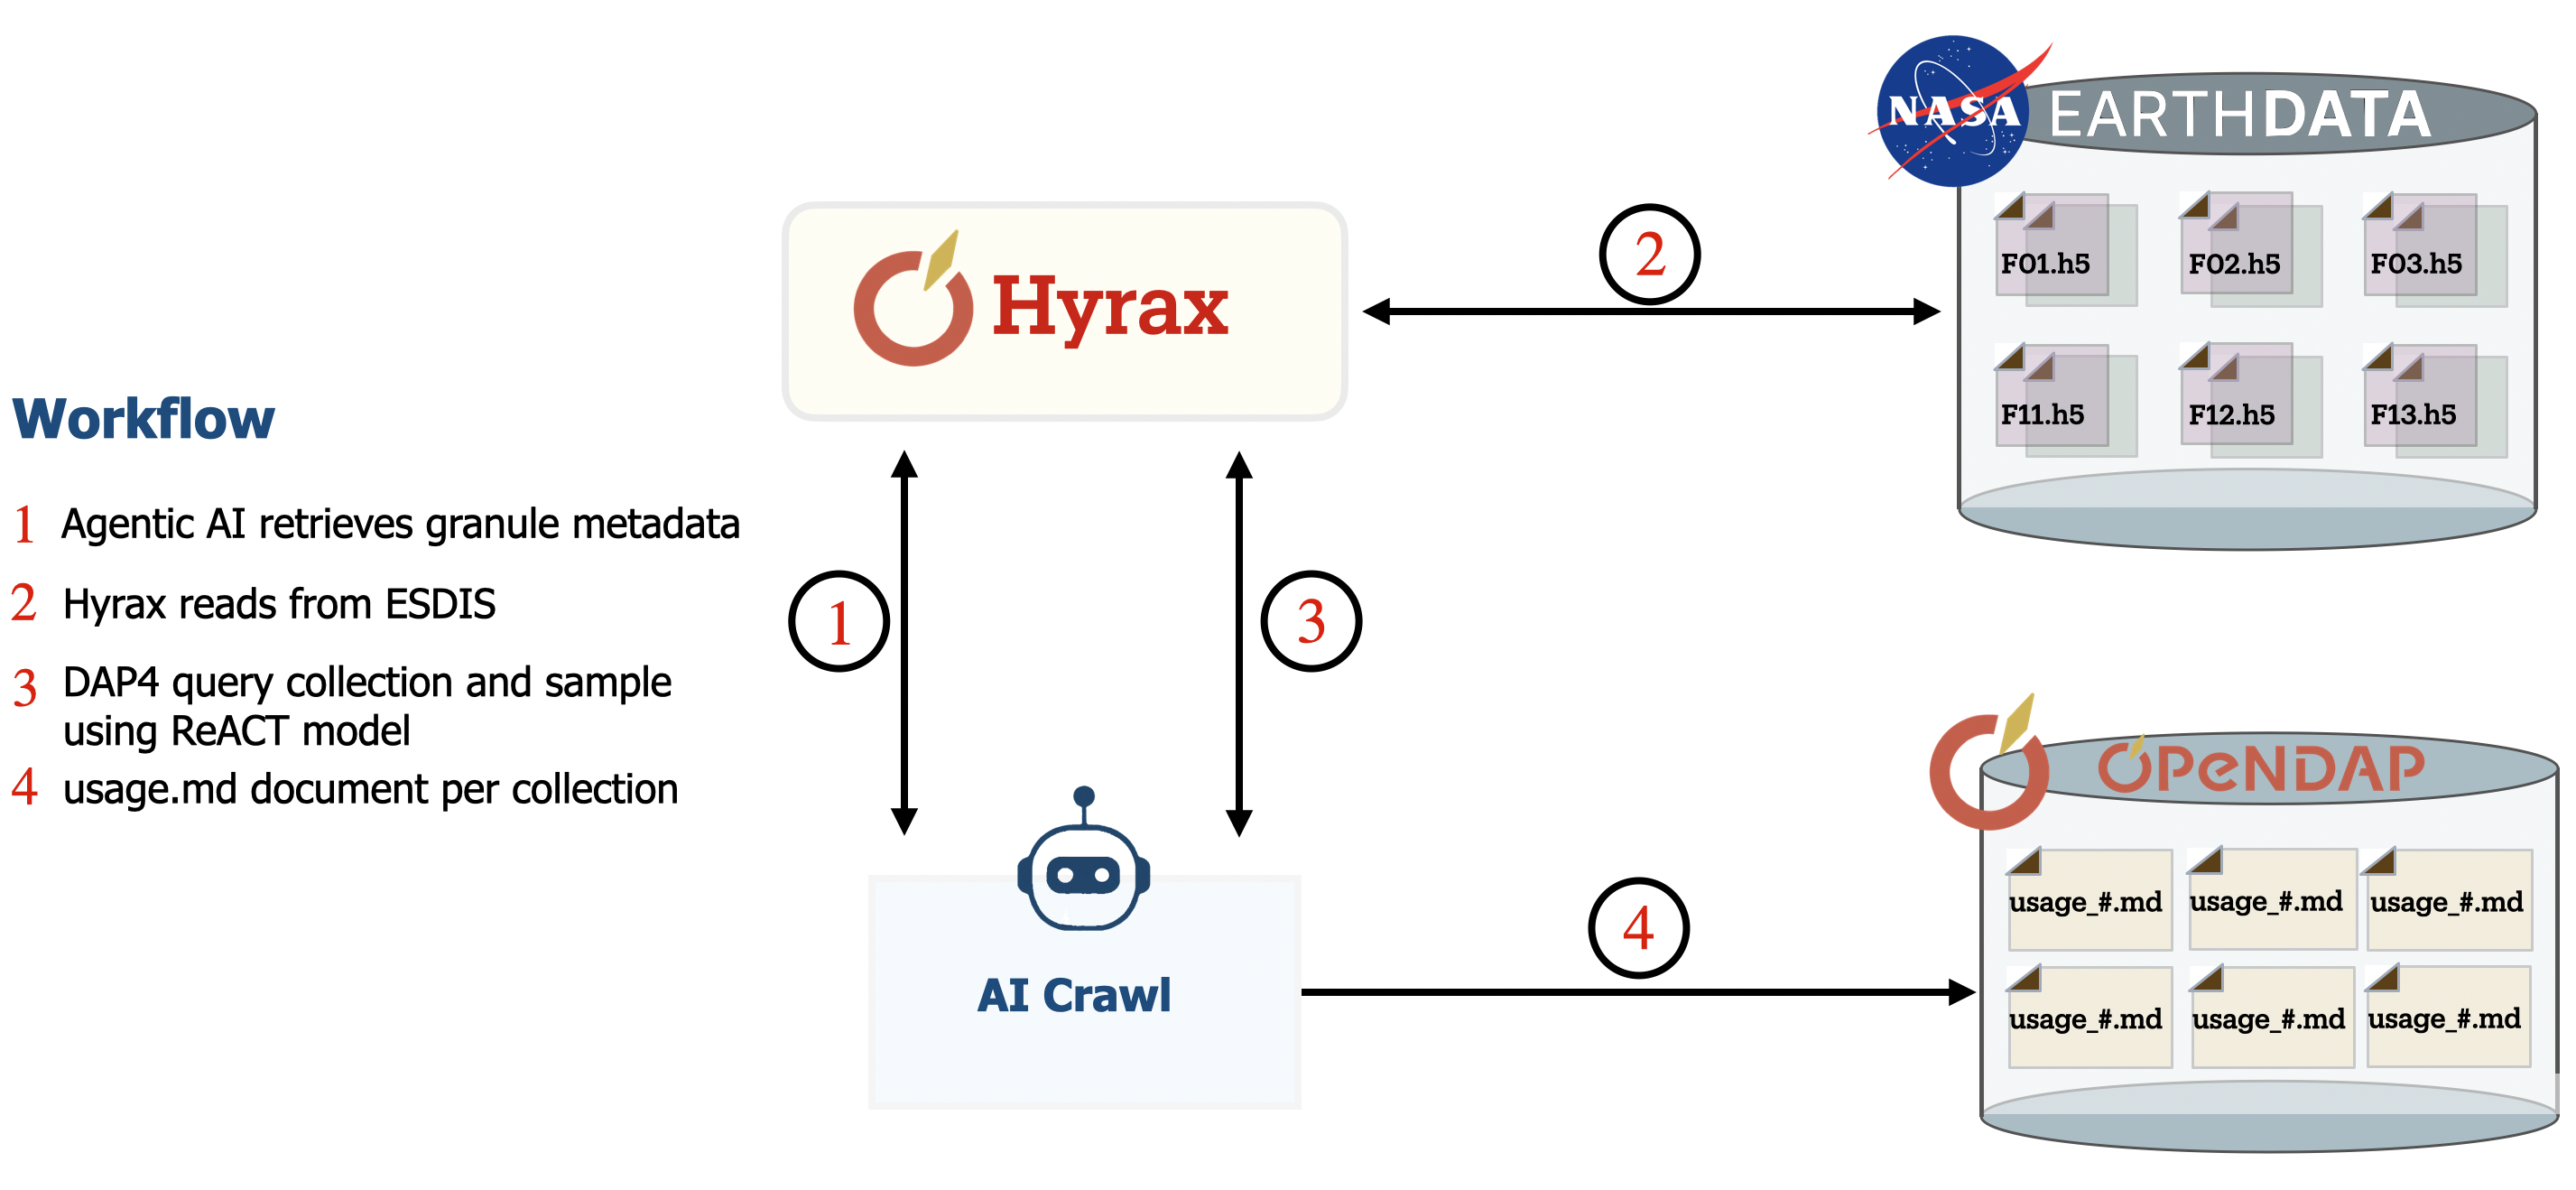
\includegraphics[width=.75\linewidth]{Figure1.png}
    \caption{Deployment architecture for the agentic system. In part 2 of the
    project, the crawler/agent will run in AWS, The
    agent will query CMR and \ac{OPeNDAP}/Hyrax and store the \texttt{usage.md}
    documents in AWS S3. In part 3 The Hyrax service will integrate the metadata
    documents into its responses.}
    \label{fig1:placeholder}
\end{figure}

Figure~\ref{fig1:placeholder} illustrates the workflow. The agent will be
configured with a schema for the \texttt{usage.md} documents and a set of tools
to execute the various tasks required for metadata introspection and validation.
The generated \texttt{usage.md} documents will be stored in an S3 bucket manged
by \ac{OPeNDAP} and separate from any of the \acs{DAAC} artifacts.

For each selected collection, the workflow will query \ac{CMR}, traverse Hyrax,
inspect \ac{DAP4} structural metadata, sample representative granules through
\acs{OPeNDAP} using tools such as \ac{PyDAP}, inspect \ac{DMR++} access
structure where available, run deterministic validators, compare evidence
across granules, and draft collection \texttt{usage.md} documents. The resulting
\texttt{usage.md} schema will include collection scope, provenance, source
identifiers, variables, units, coordinates, fill values, valid ranges, temporal
and spatial bounds, chunking and access guidance, known access issues, evidence
links, confidence labels, review status, and last-refresh time.\footnote{For
some collections, not all of this information may be relevant.}

The agent may propose inferences, but every claim must be labeled as {\em
stated}, {\em inferred}, {\em uncertain}, or {\em unsupported}. Unsupported
claims will be omitted or routed for review rather than published. At no time
with this system modify any \ac{EDC} artifact (e.g., \ac{CMR} record); only the
\texttt{usage.md} documents will be created/edited by this system.

This part of the project also adds `staleness' controls. Each \texttt{usage.md} document will include
versioning, provenance, review status, and timestamps. While out of scope for
this project, these features provide a path to future expansion to include support for
Governance and Standards. We include them here because they simplify the review
of the \texttt{usage.md} documents by a human expert.

Because \ac{DMR++} exposes chunk structure and related access information
through the \acs{OPeNDAP} interface, the guidance can also describe retrieval
strategies that avoid unnecessary reads and align requests with chunked cloud
objects where possible. That information is useful to autonomous agents and to
virtual data systems such as VirtualiZarr~\cite{nicholas_2026_virtualizarr}.

\subsection{Machine-actionable guidance for autonomous data retrieval workflows}
\label{section-2.3}

The third part of the project will make eligible \texttt{usage.md} documents
available when users access data using \ac{OPeNDAP}. Part 2 creates and validates
collection-level \texttt{usage.md} artifacts; Part 3 exposes the guidance and its
review status through existing \ac{OPeNDAP}/Hyrax responses so clients can retrieve
it in-band when they request data or metadata. This keeps the solution inside existing
\acs{OPeNDAP} service patterns and avoids creating another discovery portal.

Reviewed \texttt{usage.md} documents will be exposed through this mechanism, and
unreviewed documents may also be exposed when the agentic workflow and
deterministic checks identify no questionable claims, unresolved discrepancies,
unsupported inferences, or validation failures. Documents that contain such
flags will not be included in the \ac{OPeNDAP} responses and instead flagged for
expert review.

Nevertheless, every \texttt{usage.md} artifact, whether exposed or withheld, will
retain provenance, confidence, last-refresh information, and an explicit review
status. Exposed documents will be labeled as {\em reviewed} or {\em unreviewed with no
issues flagged}; documents withheld for review will be labeled as
review required. Existing \acs{OPeNDAP} clients will continue to
work without change, while agent-aware clients will be able to locate and use the
guidance.

\section{Deliverables}
At the end of the project, three new concrete outputs:

\begin{enumerate}
\item \textbf{A working \ac{AI}-crawlable interface prototype.} We will deliver
a Virtual Directory Interface for representative \acs{OPeNDAP}-enabled
\ac{ESDIS} collections. The prototype will show that generic
\ac{AI} clients can discover target collections, traverse collection structure,
and reach expected \ac{DAP4} service endpoints. If production deployment
approval is outside the project's control during the award period, we will
deliver the working prototype and a documented \ac{EDC} integration path.

\item \textbf{An open-source metadata-introspection repository.} We will deliver
software that crawls selected collections, queries \ac{CMR}, inspects
\acs{OPeNDAP}/Hyrax responses, samples representative granules, and drafts
evidence-linked collection guidance. The public repository will include source
code, schemas, prompts or workflow configuration, validation scripts, regression
tests, developer documentation, and reproducibility notes.

\item \textbf{Reviewed guidance, documentation, and demonstration materials.}
For collections selected with our \ac{DAAC} collaborator, we will deliver
reviewed \texttt{usage.md} files covering, as appropriate, identifiers,
variables, units, and other metadata elements described in
Section~\ref{section-2.2}. Approved guidance will be exposed through prototype
\ac{OPeNDAP}Hyrax responses, accompanied by user documentation, sample workflows,
validation results, a final report, and a presentation/demo.
\end{enumerate}

\textbf{Note}: In the deliverables above we note that the deliverables will
cover {\em selected} and/or {\em representative} collections and granules. This
is to ensure the work and the promised deliverables are achievable within the
project scope. 

\section{Validations and Path to Operations}
Our validation approach follows from the three deliverables. For Part 1, we will
validate the Virtual Directory Interface by confirming that generic \ac{AI}
clients can discover and traverse representative \acs{OPeNDAP}-enabled
collections in \ac{ESDIS} without collection-specific adaptation. Success will
be measured by fraction of the collections and granules that can be accessed.

For Part 2, we will validate the reachability of the key endpoints (i.e.,
\ac{CMR}, \acs{OPeNDAP}/Hyrax, and \ac{DMR++} documents) by the \ac{AI} agents.

In addition, we will validate
the agentic metadata-generation workflow by
comparing the generated markdown documents against authoritative sources,
including \ac{CMR} collection and granule metadata, and the results of direct
\ac{DAP4} inspection. The system will be judged on whether it produces complete,
evidence-linked metadata summaries, correctly flags uncertainty or disagreement,
and avoids asserting facts that are not supported by the data or upstream
metadata. The team has three expert validators that can review the generated documents.

For Part 3, we will validate operational usefulness by testing whether an
autonomous client can use the embedded guidance (the content of the
\texttt{usage.md} documents embedded in the response from the \ac{OPeNDAP}/Hyrax
service) to make correct data access and
subsetting requests.

Validation will also include presence of open-science products that are part of
our public GitHub repository. These include scripts, test cases, generated
sample guidance, and validation results. In addition, the \texttt{usage.md}
documents themselves will be open-science artifacts that can be reviewed by the
public and by domain experts. We will follow NASA policy/guidance on how
publicly available these documents should be.

\section{Timeline}

\subsection*{Part 1: AI-discoverable and crawlable service interfaces} 
\begin{description}
    \item [Month 1] Deploy and test the Hyrax Virtual Directory Interface
    candidate and define target validation collections. 
\end{description}

Decision point: confirm that the interface is operational (as a working
prototype).

\subsection*{Part 2: AI-assisted metadata introspection and validation} 
\begin{description}
    \item [Month 2] Design the agent workflow, evidence schema, and `usage.md` schema.
    \item [Month 3] Implement initial \ac{CMR}, \acs{OPeNDAP}/Hyrax, \ac{PyDAP}, and \ac{DMR++} tool calls.
    \item [Month 4] Generate the first `usage.md` artifacts for representative
    collections. Run expert review and revise validators based on the review. 
\end{description}
   
Decision point: Confirm that the generated metadata documents are accurate and
useful, and that the review process is effective.


\subsection*{Part 3: Machine-actionable guidance for autonomous data retrieval workflows} 
\begin{description}
    \item [Month 5] Prototype \ac{DAP4} embedding guidance (i.e., the
    information in the \texttt{usage.md} documents) in Hyrax responses.
    \item [Month 6] Validate autonomous retrieval workflows and the operational
    review path. 
\end{description}

Package the open-source artifacts, final report, and presentation/demo, and
present the working prototype as the final deliverable. 

\section{Team}

The project team combines \acs{OPeNDAP} engineering, NASA \ac{PODAAC}
operational knowledge, and physical-oceanography domain expertise. {\em James
Gallagher} will lead the project and contribute agentic \ac{AI} development and
software engineering. An {\em Dan Holloway} will contribute agentic \acs{AI}
development and software engineering. Both Holloway and Gallagher have prior
experience building \ac{AI} systems. {\em Miguel \`{A}ngel Jim\`{e}nez} will
collaborate on agentic \acs{AI} development, domain review, and testing as an
\acs{OPeNDAP}-funded contributor. Miguel has a background in machine learning
and physical oceanography.

The \ac{PODAAC}/\ac{ESDIS} connection is provided by {\em Ed Armstrong} at NASA
\ac{JPL} \acs{PODAAC}. Ed will support domain validation and testing, help select
representative collections, and provide \acs{PODAAC} operational feedback on
whether the prototype fits practical \ac{DAAC} review workflows. This gives the
work a direct validation path against NASA \acs{ESDIS} operational needs, rather
than only an \acs{OPeNDAP}-side software demonstration.

{\em Peter Cornillon} is the originator of the work described in the
\texttt{grep-dap} project (Section~\ref{section-1.1}) and will provide
consultation as needed, as well as serving as a Domain expert in Physical
Oceanography where he has published extensively.

Appendix~\ref{app-team} provides Table~\ref{tab-team}, which summarizes the team
members, effort, and contributions.


\section{Budget Summary}
\label{section-budget}
% Ideally, we should include 7% for Raytheon's markup on the cost of myself
% and Hannah. I just guessed at that and put a cap at a bit more than 186K.

\noindent 
\textbf{Note} See Appendix~\ref{app-budget} for Table~\ref{tab-budget} which summarizes the budget information.\\
\textbf{Indirect costs} There are no indirect costs added to the
budget since payment is through the existing \ac{ESDIS} contract
(EED3\footnote{NASA Earth Observing System Data and Information System Evolution and
Development-3} for \acs{OPeNDAP}).\\
\textbf{Hardware procurement} No hardware procurement is requested; existing
infrastructure will be utilized.\\
\textbf{Travel} Travel is excluded from the budget.\\
\textbf{Other direct costs} Other direct costs include cloud compute resources
for AI model and inference, estimated at \$10,000 over the project
duration. This estimate is based on OpenAI model costs, LangChain usage and AWS
cloud compute for testing.\\
\textbf{Personnel} Personnel costs are based on the estimated hours and hourly
rates for the project team members, as detailed in the budget table above. The
total personnel cost is \$173,177. {\em James Gallagher} will lead the project
and provide guidance on the Hyrax/\acs{OPeNDAP} architecture, Virtual Directory
interface, agentic AI development and software engineering. {\em Dan Holloway}
will contribute to agentic AI development and software engineering. {\em Ed
Armstrong} will provide \ac{DAAC}/domain validation, \ac{PODAAC} operational
feedback, representative collection selection and testing support. {\em Miguel
\`{A}ngel Jim\`{e}nez} will be funded by \ac{OPeNDAP} to collaborate with an
{\em Dan Holloway} on agentic \ac{AI} development and use of \ac{PyDAP} as part
of his role in \ac{OPeNDAP} as the Scientific Community Director. {\em Peter
Cornillon} will contribute unfunded domain validation and testing as a
collaborator at \ac{OPeNDAP} and the University of Rhode Island. 

\pagebreak

\appendix

\section{Team}
\label{app-team}
\begin{table}[htbp]
  \centering
  \caption{Team members and their contributions to the project.}
  \label{tab-team}
\begin{minipage}
{\linewidth}
\begin{tabular}{|l|l|p{3.5in}|}
\hline
Name & Effort & Role / Contribution \\
\hline
James Gallagher & 2 months & Project lead; agentic \ac{AI} development; software engineering \\
\hline
Dan Holloway & 2 months & Agentic \ac{AI} development; software engineering \\
\hline
Ed Armstrong & 1 month & Domain expert and testing; key collaborator at \ac{PODAAC} \\
\hline
Miguel \`{A}ngel Jim\`{e}nez & 2 months\footnote{Funded by \ac{OPeNDAP}} & Agentic \ac{AI} development, domain expert and testing; collaborator at \acs{OPeNDAP} \\
\hline
Peter Cornillon & Unfunded & Domain expert and testing; collaborator at
\ac{OPeNDAP} and the University of Rhode Island \\
\hline
\end{tabular}
\end{minipage}
\end{table}


\section{Budget table}
\label{app-budget}
\begin{table}[htbp]
  \centering
  \caption{Summarized budget information for the project.}
  \label{tab-budget}
\begin{tabular}{|l|l|l|l|l|}

\hline
Who & Hourly rate & Months & Cost \\
\hline
James Gallagher & \$220.15 & 2 & \$73,530 \\
\hline
Dan Holloway & \$199.07 & 2 & \$66,489 \\
\hline
Ed Armstrong & See budget in Appendix~\ref{app-jpl-budget} & 1 & \$33,158 \\
\hline
 & Monthly cost & &  \\
\hline
Compute & \$2,500.00 & 4 & \$10,000 \\
\hline
Tooling & n/a & & n/a \\
\hline
 &  &  &  \\
\hline
Total &  &  & \$183,177 \\
\hline
\end{tabular}
\end{table}

\clearpage % Ensures figures/tables from the previous section are output
\section{Budget details for Ed Armstrong at JPL}
\label{app-jpl-budget}
\begin{figure}[htbp]
    \centering
    % \caption{Budget details for Ed Armstrong at JPL.}
    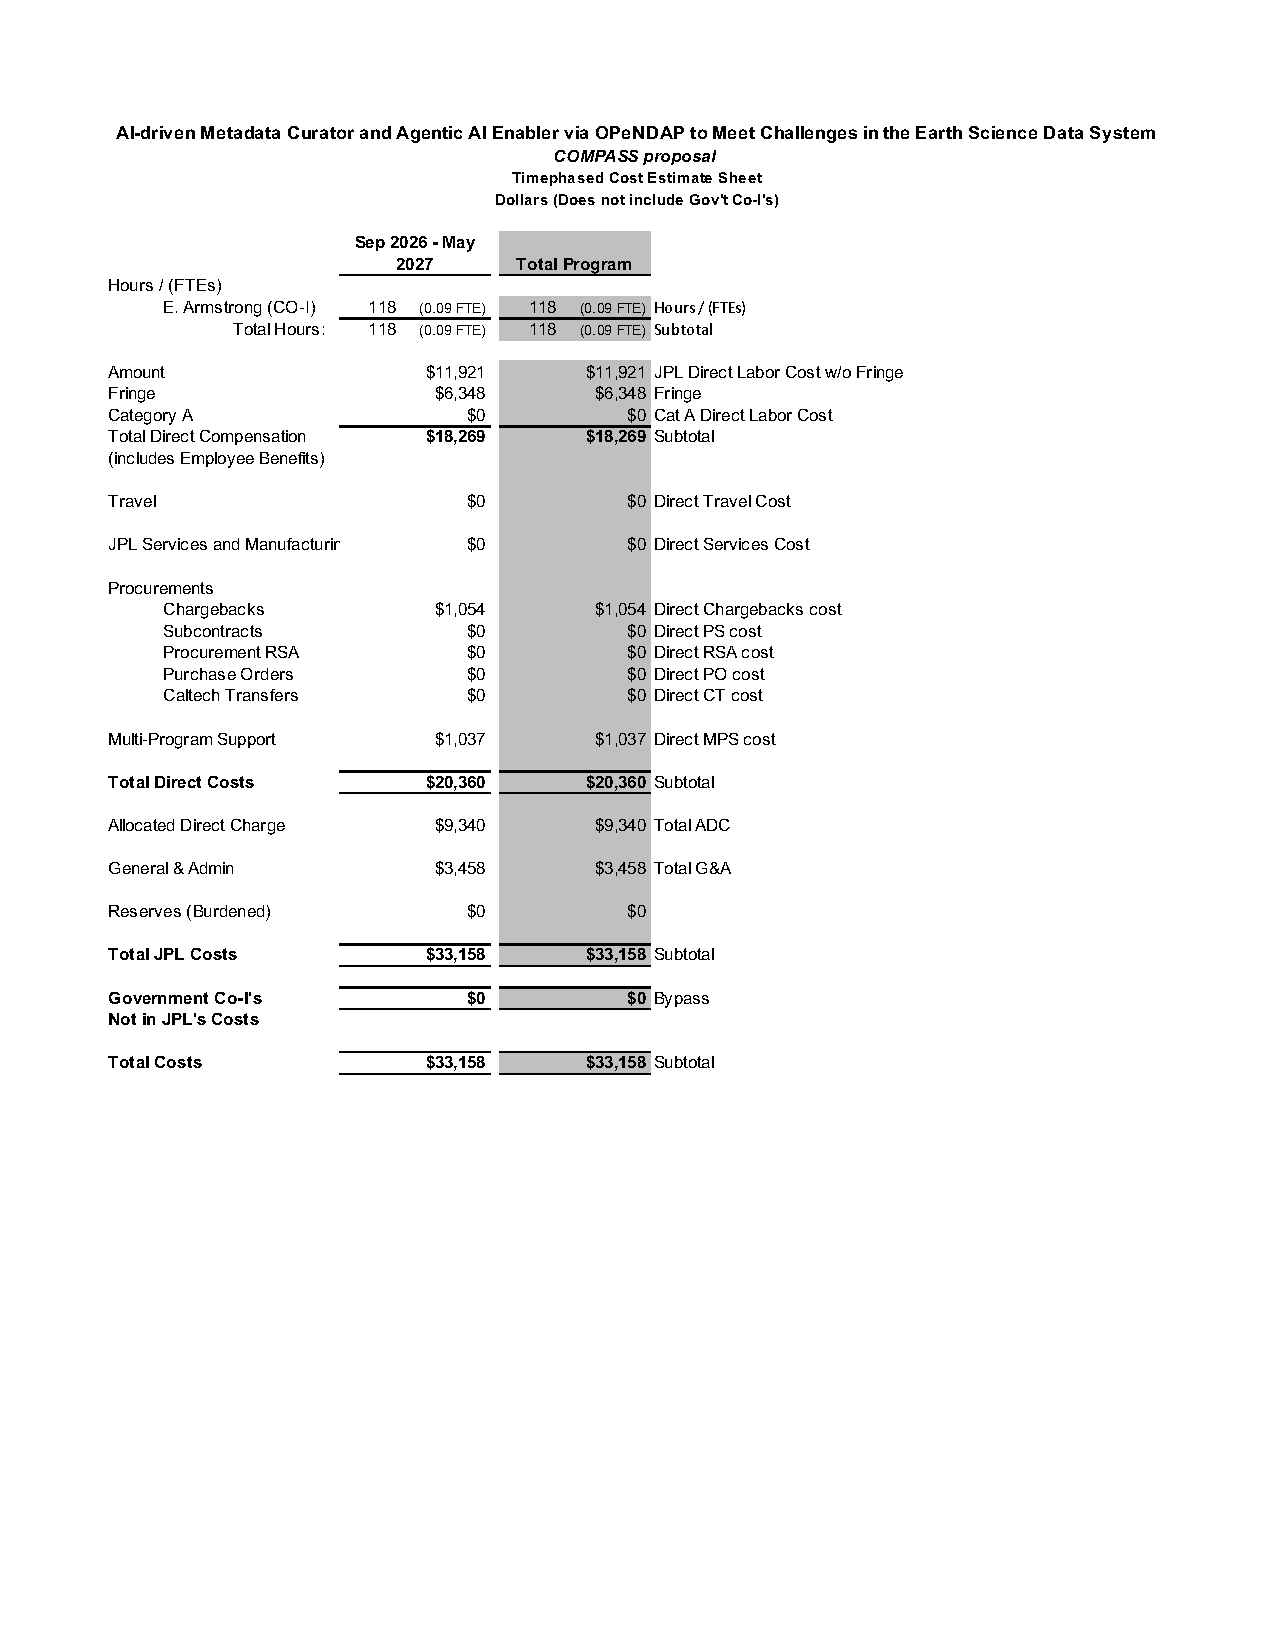
\includepdf[
    pages=1, % Inserts only the first page. Use 'pages=-' for all pages
    pagecommand={\thispagestyle{plain}}, % Standard page numbers
    offset=0mm -10mm, % Adjusts the (x,y) position of the included page    
    scale=0.9, % Scales the PDF down slightly to fit LaTeX margins
    frame=false % Set to true to draw a border around the included page
    ]{budgets/Ed-Armstrong-v2.pdf}
\end{figure}    

\clearpage % Ensures figures/tables from the previous section are output

\bibliography{references}

\end{document}
